\documentclass[a4paper,12pt]{jsarticle}
\usepackage[dvipdfmx,margin=24mm]{geometry}
\usepackage[dvipdfmx]{graphicx}
\usepackage{amsmath,amssymb,amsthm}
\usepackage{enumitem}
\usepackage{tikz}
\usepackage{pgfplots}
\usepackage{float}

\pgfplotsset{compat=1.18}

\setlength{\parindent}{0pt}
\setlength{\parskip}{0.35em}
\setlist[itemize]{leftmargin=2em,itemsep=0.2em,topsep=0.3em}
\setlist[enumerate]{leftmargin=2em,itemsep=0.4em,topsep=0.3em}

\pgfplotsset{
  taylorplot/.style={
    width=0.92\linewidth,
    height=0.52\linewidth,
    axis lines=middle,
    xlabel={$x$},
    ylabel={$y$},
    grid=both,
    grid style={gray!20},
    minor tick num=1,
    tick label style={font=\small},
    label style={font=\small},
    legend cell align=left,
    legend style={
      draw=gray!40,
      fill=white,
      fill opacity=0.9,
      text opacity=1,
      font=\small
    },
    samples=200
  }
}

\theoremstyle{definition}
\newtheorem*{definition}{定義}
\newtheorem*{theorem}{定理}

\begin{document}

\begin{center}
{\LARGE 数学1A 第5回レジュメ}\\[0.4em]
テイラー展開とテイラー多項式
\end{center}

\section{形式的なテイラー展開}

\begin{definition}[形式的なテイラー展開]
関数 $f$ が点 $a$ で何回でも微分可能であるとする。このとき
\[
\sum_{k=0}^{\infty}\frac{f^{(k)}(a)}{k!}(x-a)^k
\]
を，$f$ の $a$ における形式的なテイラー展開という。
\end{definition}

ここで「形式的」とは，この無限和が収束することや，収束した値が $f(x)$ と一致することをまだ主張しない，という意味である。
微分の値 $f(a),f'(a),f''(a),\dots$ から作られる「候補」として考える。

\section{テイラー多項式}

\begin{definition}[テイラー多項式]
$f$ が点 $a$ で $n$ 回微分可能であるとする。このとき
\[
T_n(x)=\sum_{k=0}^{n}\frac{f^{(k)}(a)}{k!}(x-a)^k
\]
を，$f$ の $a$ における $n$ 次テイラー多項式という。
\end{definition}

テイラー多項式は有限和なので，収束の問題はない。また，$0\leq j\leq n$ に対して
\[
T_n^{(j)}(a)=f^{(j)}(a)
\]
が成り立つ。つまり，$T_n(x)$ は点 $a$ で $f(x)$ と $n$ 階微分まで同じ値を持つ多項式である。

\section{例}

\subsection*{例1. $f(x)=x^2$, $a=0$}

$f(0)=0$, $f'(0)=0$, $f''(0)=2$ であり，$k\geq 3$ では $f^{(k)}(0)=0$ である。したがって
\[
T_0(x)=0,\qquad
T_1(x)=0,\qquad
T_2(x)=x^2,\qquad
T_3(x)=x^2.
\]

\begin{figure}[H]
\centering
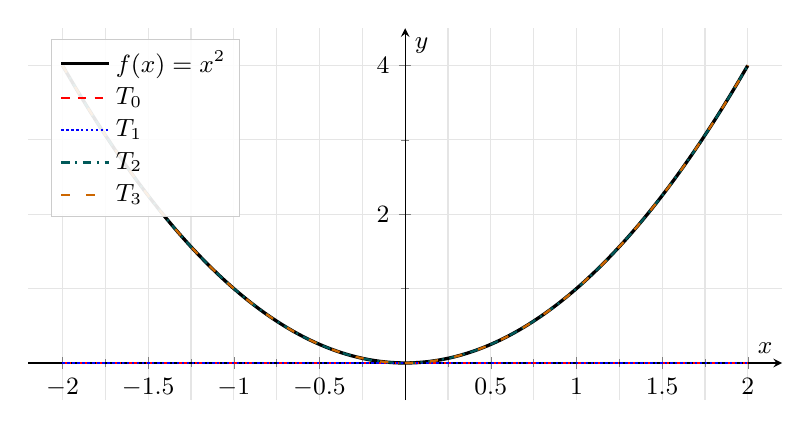
\begin{tikzpicture}
\begin{axis}[
  taylorplot,
  xmin=-2.2,xmax=2.2,
  ymin=-0.5,ymax=4.5,
  legend pos=north west
]
\addplot[black, very thick, domain=-2:2] {x^2};
\addlegendentry{$f(x)=x^2$}
\addplot[red, thick, dashed, domain=-2:2] {0};
\addlegendentry{$T_0$}
\addplot[blue, thick, densely dotted, domain=-2:2] {0};
\addlegendentry{$T_1$}
\addplot[teal!70!black, thick, dashdotted, domain=-2:2] {x^2};
\addlegendentry{$T_2$}
\addplot[orange!80!black, thick, loosely dashed, domain=-2:2] {x^2};
\addlegendentry{$T_3$}
\end{axis}
\end{tikzpicture}
\caption{$f(x)=x^2$ と $a=0$ におけるテイラー多項式。$T_0=T_1$，$T_2=T_3=f$ である。}
\end{figure}

\subsection*{例2. $f(x)=\log x$, $a=1$}

$f(1)=0$ であり，$k\geq 1$ に対して
\[
f^{(k)}(x)=(-1)^{k-1}\frac{(k-1)!}{x^k}
\]
である。よって
\[
T_n(x)=\sum_{k=1}^{n}(-1)^{k-1}\frac{(x-1)^k}{k}
\]
となる。ただし $T_0(x)=0$ とする。特に
\[
\begin{aligned}
T_0(x)&=0,\\
T_1(x)&=x-1,\\
T_2(x)&=(x-1)-\frac{(x-1)^2}{2},\\
T_3(x)&=(x-1)-\frac{(x-1)^2}{2}+\frac{(x-1)^3}{3},\\
T_4(x)&=(x-1)-\frac{(x-1)^2}{2}+\frac{(x-1)^3}{3}-\frac{(x-1)^4}{4}.
\end{aligned}
\]

\begin{figure}[H]
\centering
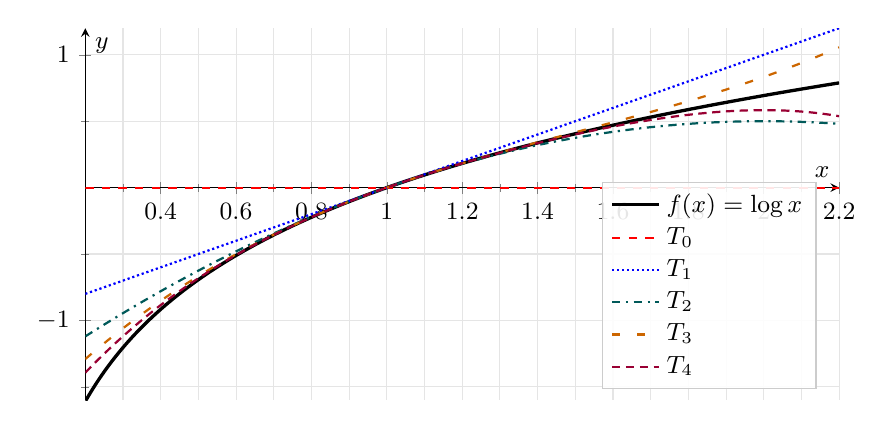
\begin{tikzpicture}
\begin{axis}[
  taylorplot,
  xmin=0.2,xmax=2.2,
  ymin=-1.6,ymax=1.2,
  legend pos=south east
]
\addplot[black, very thick, domain=0.2:2.2] {ln(x)};
\addlegendentry{$f(x)=\log x$}
\addplot[red, thick, dashed, domain=0.2:2.2] {0};
\addlegendentry{$T_0$}
\addplot[blue, thick, densely dotted, domain=0.2:2.2] {x-1};
\addlegendentry{$T_1$}
\addplot[teal!70!black, thick, dashdotted, domain=0.2:2.2] {(x-1)-((x-1)^2)/2};
\addlegendentry{$T_2$}
\addplot[orange!80!black, thick, loosely dashed, domain=0.2:2.2] {(x-1)-((x-1)^2)/2+((x-1)^3)/3};
\addlegendentry{$T_3$}
\addplot[purple!80!black, thick, densely dashed, domain=0.2:2.2] {(x-1)-((x-1)^2)/2+((x-1)^3)/3-((x-1)^4)/4};
\addlegendentry{$T_4$}
\end{axis}
\end{tikzpicture}
\caption{$f(x)=\log x$ と $a=1$ におけるテイラー多項式。中心 $x=1$ の近くで近似がよくなる。}
\end{figure}

\subsection*{例3. $f(x)=\sin x$, $a=0$}

$\sin x$ の導関数は周期的に変わるので，$0$ における偶数階微分はすべて $0$ である。したがって
\[
T_n(x)=\sum_{0\leq 2k+1\leq n}(-1)^k\frac{x^{2k+1}}{(2k+1)!}
\]
である。$n=1,\dots,7$ では
\[
\begin{aligned}
T_1(x)&=x,\\
T_2(x)&=x,\\
T_3(x)&=x-\frac{x^3}{3!},\\
T_4(x)&=x-\frac{x^3}{3!},\\
T_5(x)&=x-\frac{x^3}{3!}+\frac{x^5}{5!},\\
T_6(x)&=x-\frac{x^3}{3!}+\frac{x^5}{5!},\\
T_7(x)&=x-\frac{x^3}{3!}+\frac{x^5}{5!}-\frac{x^7}{7!}.
\end{aligned}
\]

\begin{figure}[H]
\centering
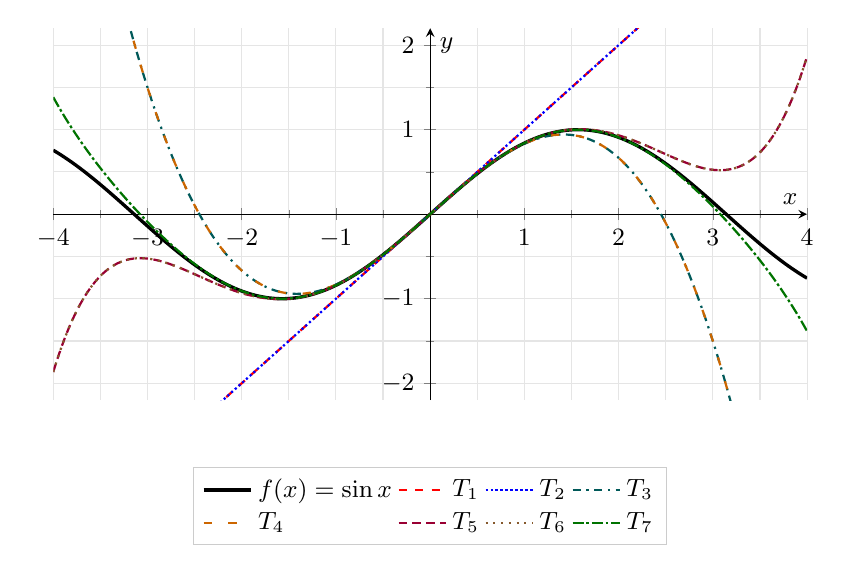
\begin{tikzpicture}
\begin{axis}[
  taylorplot,
  xmin=-4,xmax=4,
  ymin=-2.2,ymax=2.2,
  legend style={
    at={(0.5,-0.18)},
    anchor=north,
    legend columns=4,
    draw=gray!40,
    fill=white,
    font=\small
  }
]
\addplot[black, very thick, domain=-4:4] {sin(deg(x))};
\addlegendentry{$f(x)=\sin x$}
\addplot[red, thick, dashed, domain=-4:4] {x};
\addlegendentry{$T_1$}
\addplot[blue, thick, densely dotted, domain=-4:4] {x};
\addlegendentry{$T_2$}
\addplot[teal!70!black, thick, dashdotted, domain=-4:4] {x-x^3/6};
\addlegendentry{$T_3$}
\addplot[orange!80!black, thick, loosely dashed, domain=-4:4] {x-x^3/6};
\addlegendentry{$T_4$}
\addplot[purple!80!black, thick, densely dashed, domain=-4:4] {x-x^3/6+x^5/120};
\addlegendentry{$T_5$}
\addplot[brown!70!black, thick, dotted, domain=-4:4] {x-x^3/6+x^5/120};
\addlegendentry{$T_6$}
\addplot[green!45!black, thick, dash pattern=on 4pt off 1pt on 1pt off 1pt, domain=-4:4] {x-x^3/6+x^5/120-x^7/5040};
\addlegendentry{$T_7$}
\end{axis}
\end{tikzpicture}
\caption{$f(x)=\sin x$ と $a=0$ におけるテイラー多項式。$T_1=T_2$，$T_3=T_4$，$T_5=T_6$ である。}
\end{figure}

\section{テイラーの定理}

\begin{theorem}[テイラーの定理]
$I$ を区間とし，$a,x\in I$ とする。$f$ が $a$ と $x$ の間で $n+1$ 回連続的微分可能であるとき，ある $\xi$ が $a$ と $x$ の間に存在して
\[
f(x)=T_n(x)+\frac{f^{(n+1)}(\xi)}{(n+1)!}(x-a)^{n+1}
\]
が成り立つ。ただし
\[
T_n(x)=\sum_{k=0}^{n}\frac{f^{(k)}(a)}{k!}(x-a)^k
\]
である。
\end{theorem}

テイラーの定理は，関数 $f(x)$ とテイラー多項式 $T_n(x)$ の差を具体的に表している。剰余項を
\[
R_n(x)=f(x)-T_n(x)
\]
とおくと
\[
R_n(x)=\frac{f^{(n+1)}(\xi)}{(n+1)!}(x-a)^{n+1}
\]
である。したがって，$a$ と $x$ の間で
\[
|f^{(n+1)}(t)|\leq M
\]
が成り立つなら
\[
|f(x)-T_n(x)|\leq \frac{M}{(n+1)!}|x-a|^{n+1}
\]
と評価できる。

この評価から，$x$ が $a$ に近いほど誤差は小さくなりやすいことが分かる。また，テイラー多項式は単に形が似ている多項式ではなく，微分の情報を $a$ に集めて作った近似であり，その誤差も定理によって管理できる。

\end{document}
